\documentclass[xcolor=dvipsnames, compress]{beamer}
\usetheme{Berlin}
\setbeamertemplate{footline}[frame number]
\setbeamertemplate{section in toc}[sections numbered]
\setbeamertemplate{subsection in toc}[sections numbered]
\setbeamertemplate{navigation symbols}{} 
\setbeamercovered{transparent}
\usepackage{graphicx}
\usepackage{hhline}
\usepackage{appendixnumberbeamer}
\usepackage{amsmath}
\definecolor{maincolor}{rgb}{0.6, 0.4, 0.7}
\usecolortheme[named = maincolor]{structure}
\renewcommand{\arraystretch}{1.5}

\title{Marriage Bars and Teacher Pay}
\author{Amy Kim and Carolyn Tsao}
\date{March 20, 2023}

\begin{document}
\begin{frame}[plain]
    \titlepage
\end{frame}

\begin{frame}
    \frametitle{Marriage Bars: Summary of Descriptive Evidence}
        \begin{itemize}
            \item Change in \% female teachers who are single from 1900 - 1940: shifts from close to 100\% in most places to much lower levels (70\%) nationally.
            \item De-trending using \% female secretaries who are single preserves trend.
            \item Comparison of histograms between Southern states that introduced legislation lifting marriage bans for teachers in 1938 (KY, NC, DC) vs. those that did not (all others) suggests that legislation had some bite.
        \end{itemize}
\end{frame}

\begin{frame}
    \frametitle{Identification Strategy}
    Event study DiD framework:    

        \begin{eqnarray}
        y_{ct} = \alpha_t + \beta_{s(c)} + \sum_{k \in \{00, 10, 20, 40\}} \gamma_k \times \text{Treat}_c \times \text{Year}_{k=t} + \varepsilon_{ct}
        \end{eqnarray}
        
        where $y_{ct}$ is the share of female teachers who are unmarried in county $c$ in year $t$, $\alpha_t$ captures year fixed effects, $\beta_{s(c)}$ captures state fixed effects, and $T_c$ is an indicator for whether the county's state lifted the marriage ban through legislation between 1930 and 1940 (i.e. KY, NC, DC).
        
\end{frame}

\begin{frame}
    \frametitle{Event Study Plot}
    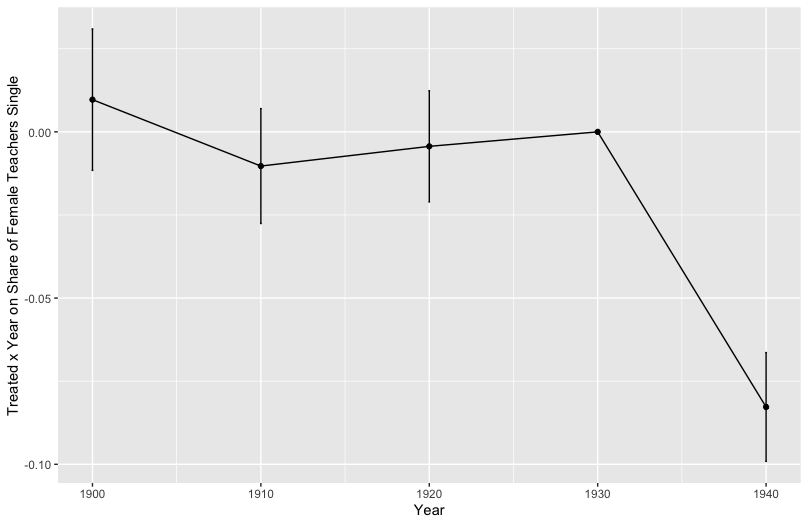
\includegraphics[width=\textwidth]{../figures/did_plot.png}
\end{frame}
\end{document}